\hypertarget{inroduction}{%
\chapter{Introduction}\label{sec:introduction}}
\thispagestyle{fancy}

The emerging applications, such as \gls{ar}/\gls{vr}, autonomous driving, mission critical \gls{iot} applications, and others, require extreme low latency of \gls{ai} decision feedback. The conventional approach is sending the sensor data, e.g., images, to the central cloud or data center to perform advanced \gls{ml} algorithms and send the results, e.g., object detection, classification, back to the end mobile devices. The conventional cloud-centric \gls{ml} framework cannot fulfill the stringent requirements of these emerging applications. \gls{mec} is a new computing paradigm which brings the computing units from the core of the network to the network edge. \gls{mec} has many benefits such as lower communication latency, higher reliability and resiliency, better security and privacy, scalability and context-awareness and others. Pushing \gls{ai} to the Edge is also known as Edge \gls{ai} or \gls{ei}.

\section{Edge Intelligence}

The primary objective of \gls{ei} is to enable intelligence for mobile and \gls{iot} application, by reducing inference latency, energy consumption and memory footprint. Progress within \gls{ai} have been pushed by the achievement in tasks using \gls{dnn}, however deployment of \gls{dnn} in real applications have been limited to the cloud, as \gls{dnn} are computationally expensive and these \gls{dnn}s are getting deeper. The tendency are exemplified by the winner of ImageNet Challenge \cite{russakovsky_imagenet_2015}, that within a time span of four years the number of layers have grown from 8 to 152 layers. This have hindered development of intelligent mobile and \gls{iot} applications. Pushing execution of \gls{dnn}  to the edge allow for flexible execution of \gls{dnn}-based applications and services. Edge-centric architectures can be categories into four main modes \cite{zhou_edge_2019}.

\begin{figure}
	\centering
	\captionsetup[subfigure]{justification=centering}
	\subfloat[Device-based\label{fig:device-based}]{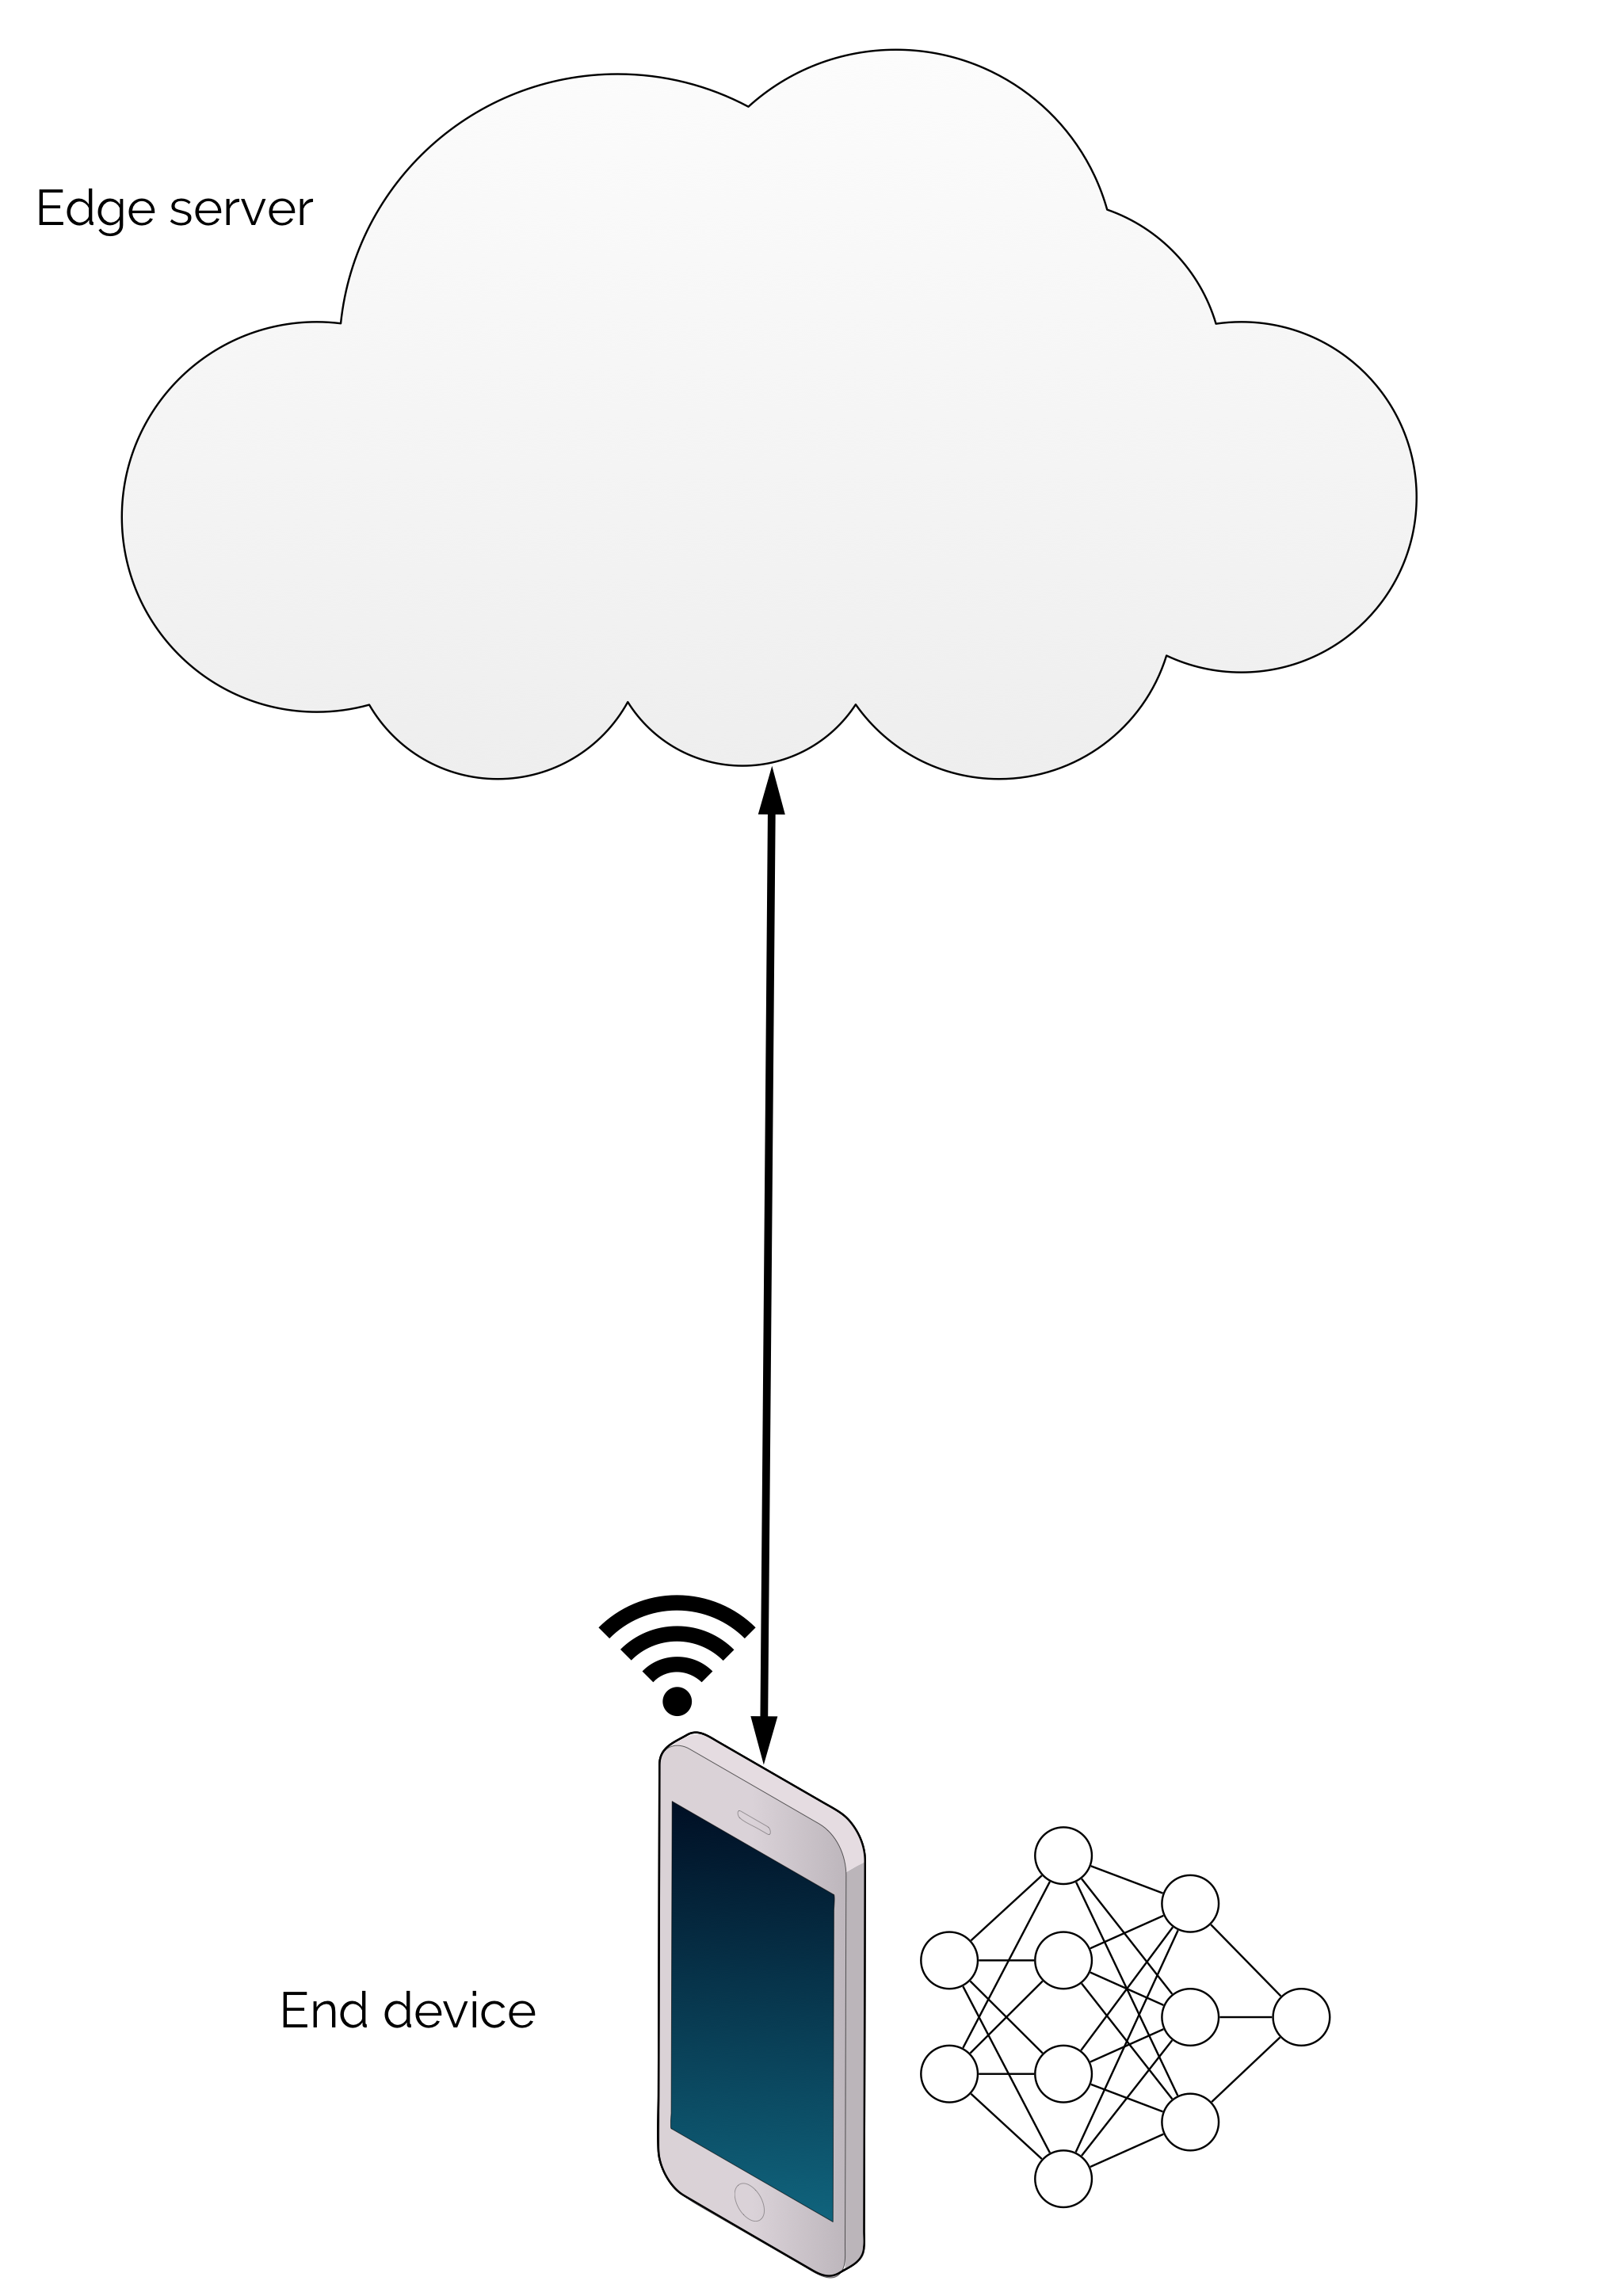
\includegraphics[width=.2\linewidth]{figures/models/device}}
	\subfloat[Edge-based\label{fig:edge-based}]{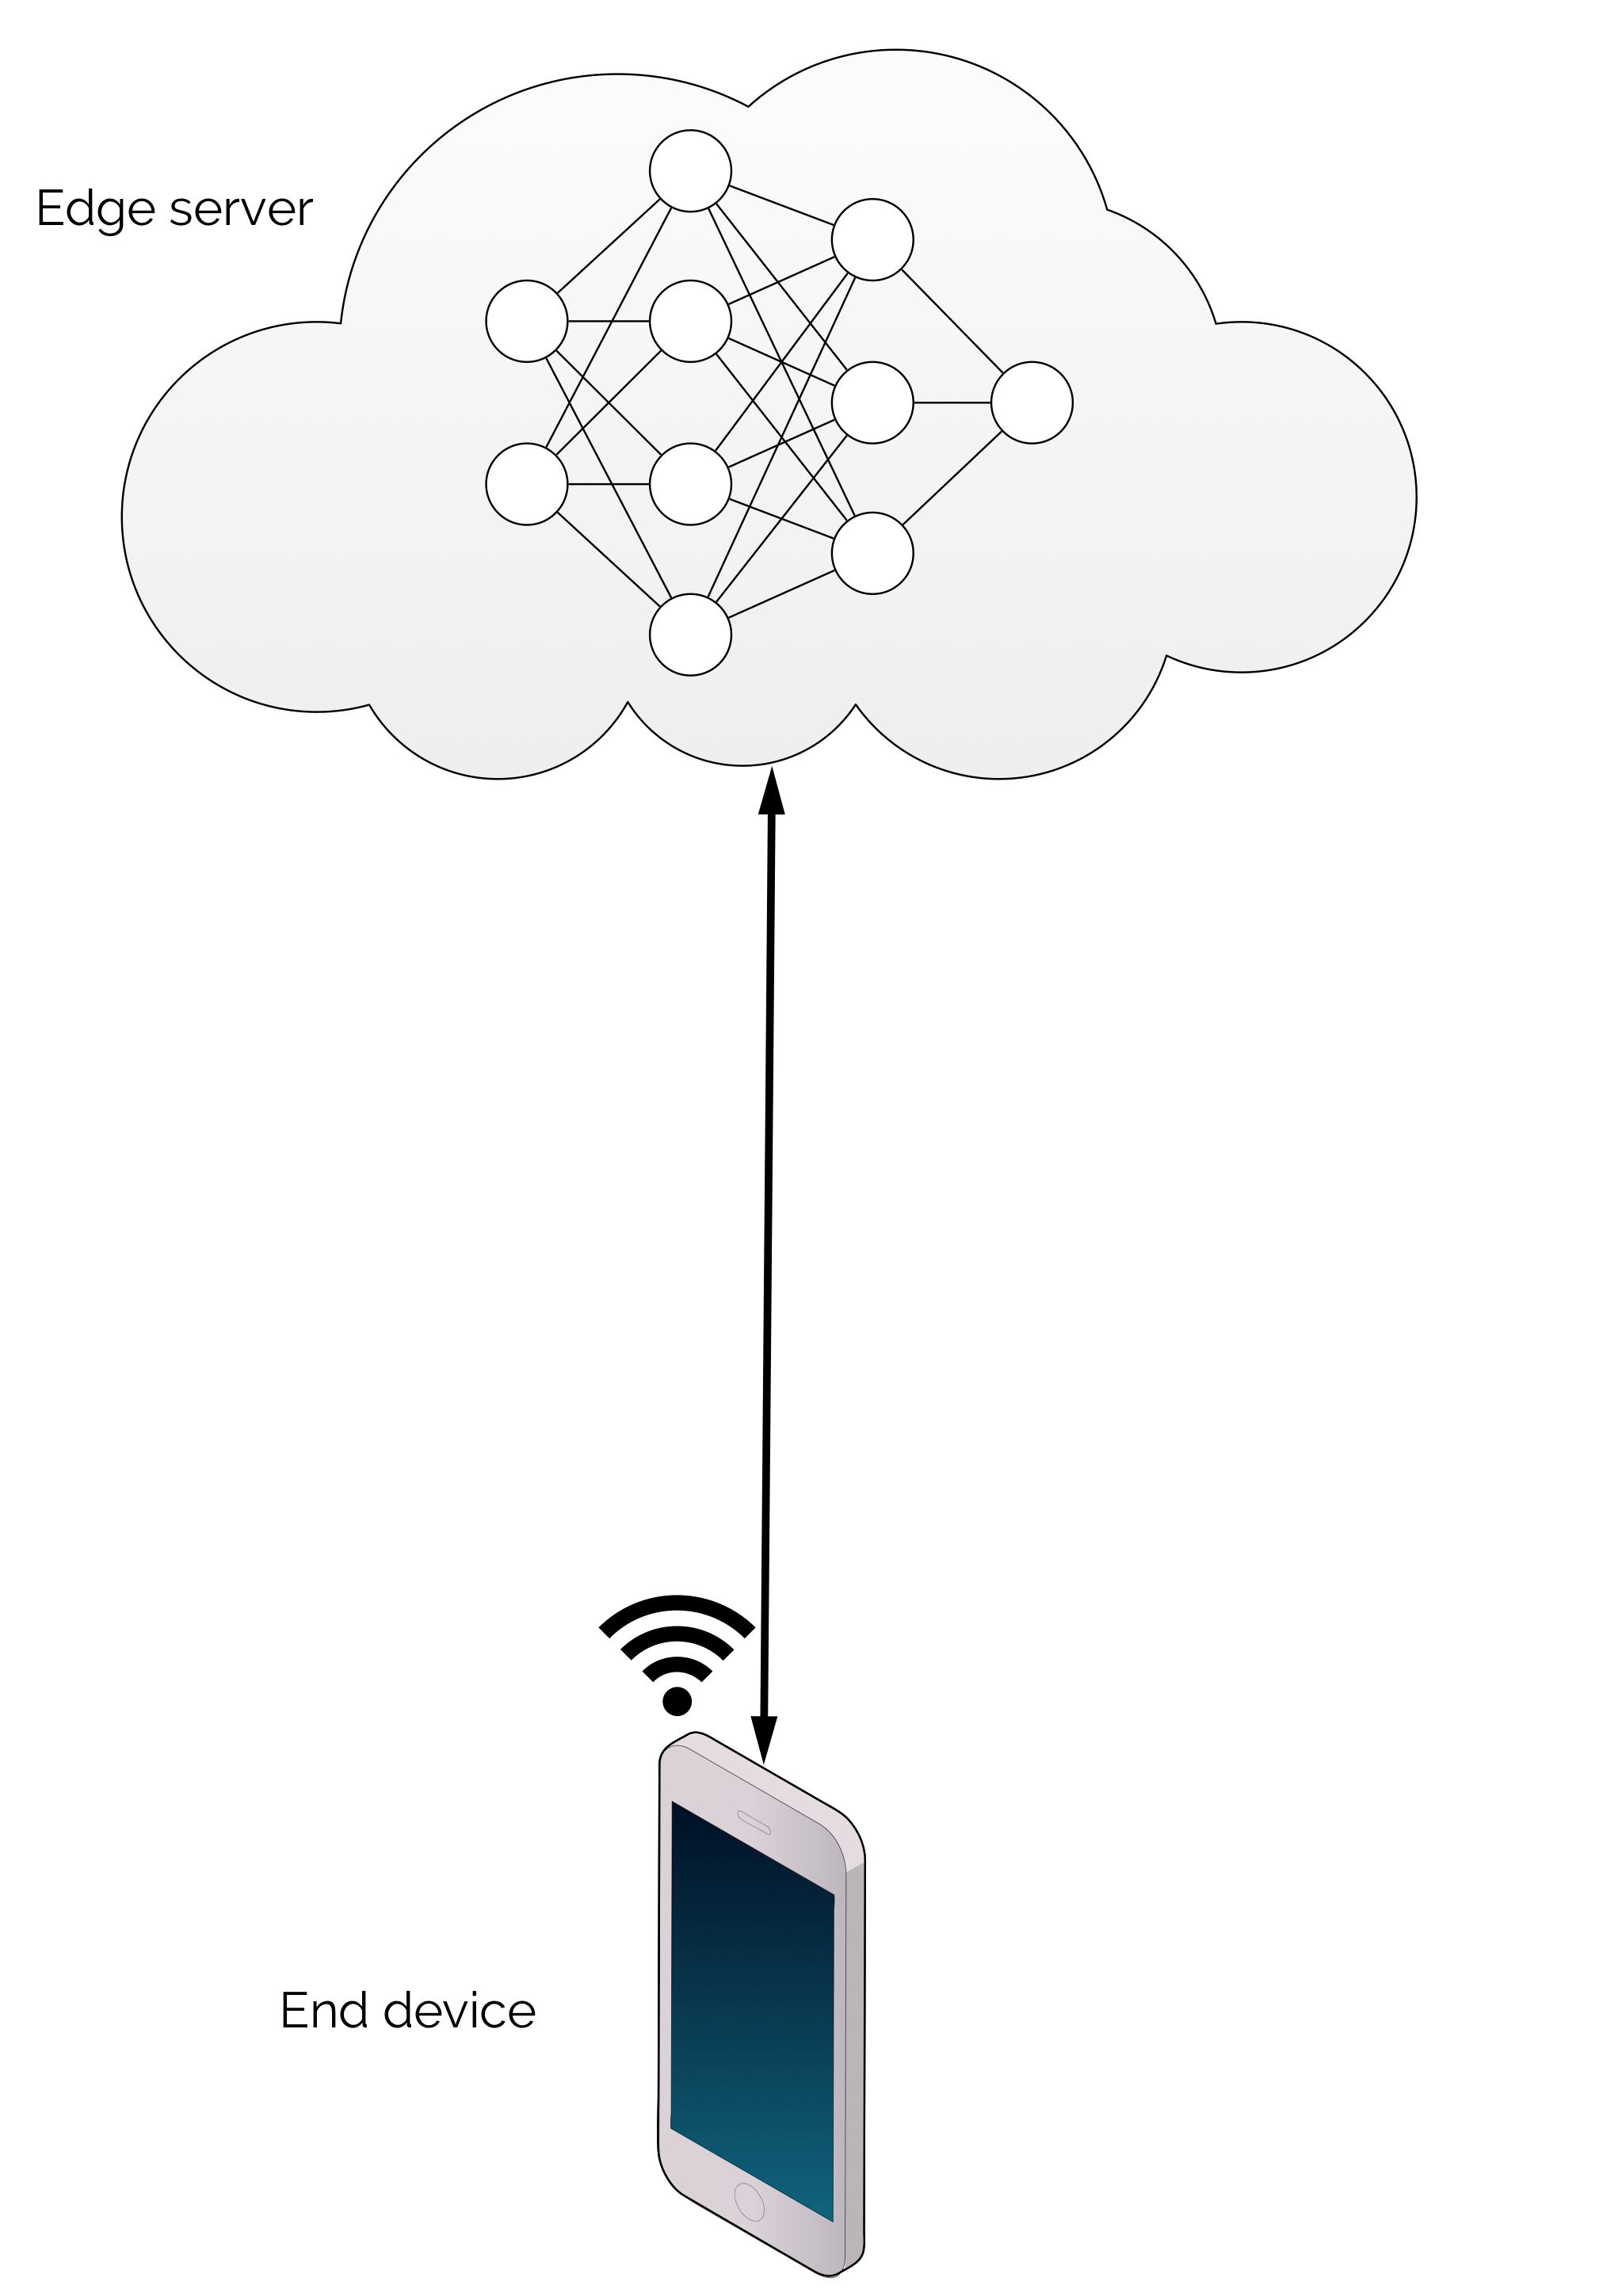
\includegraphics[width=.2\linewidth]{figures/models/edge}}
	\subfloat[Edge-Device mode\label{fig:edge-device-mode}]{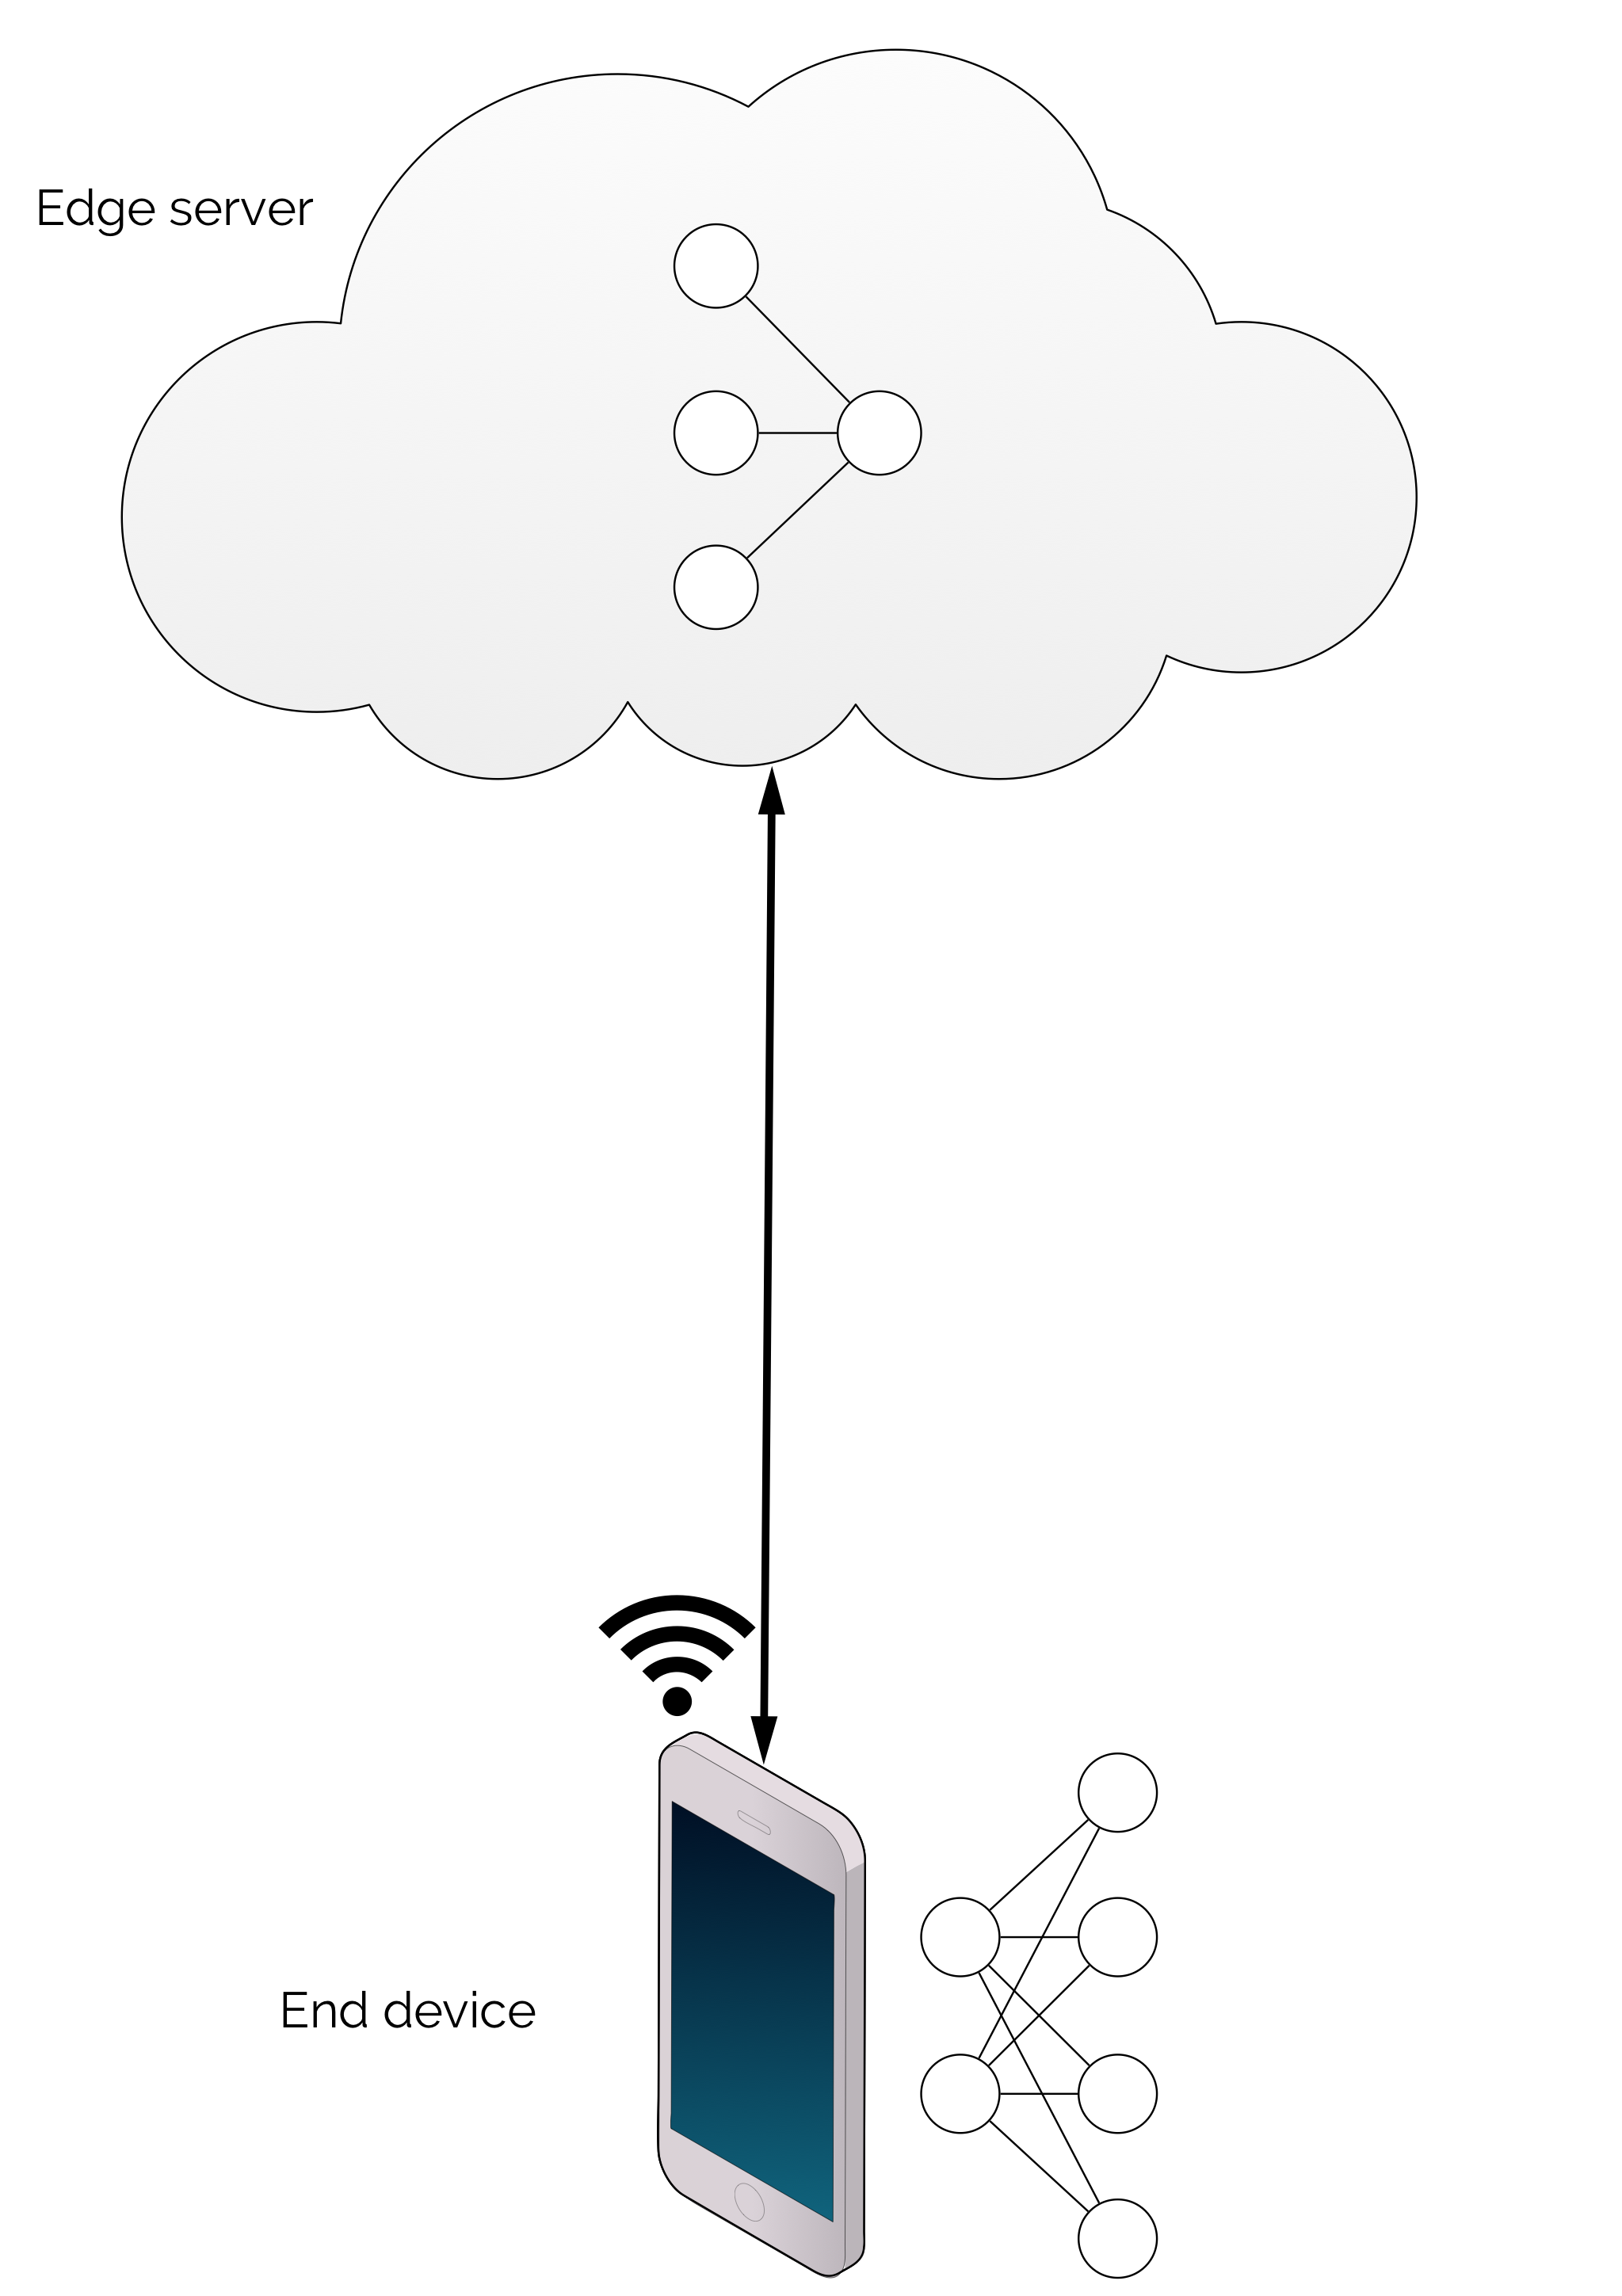
\includegraphics[width=.2\linewidth]{figures/models/edge_device}}
	\subfloat[Edge-Cloud mode\label{fig:edge-cloud-mode}]{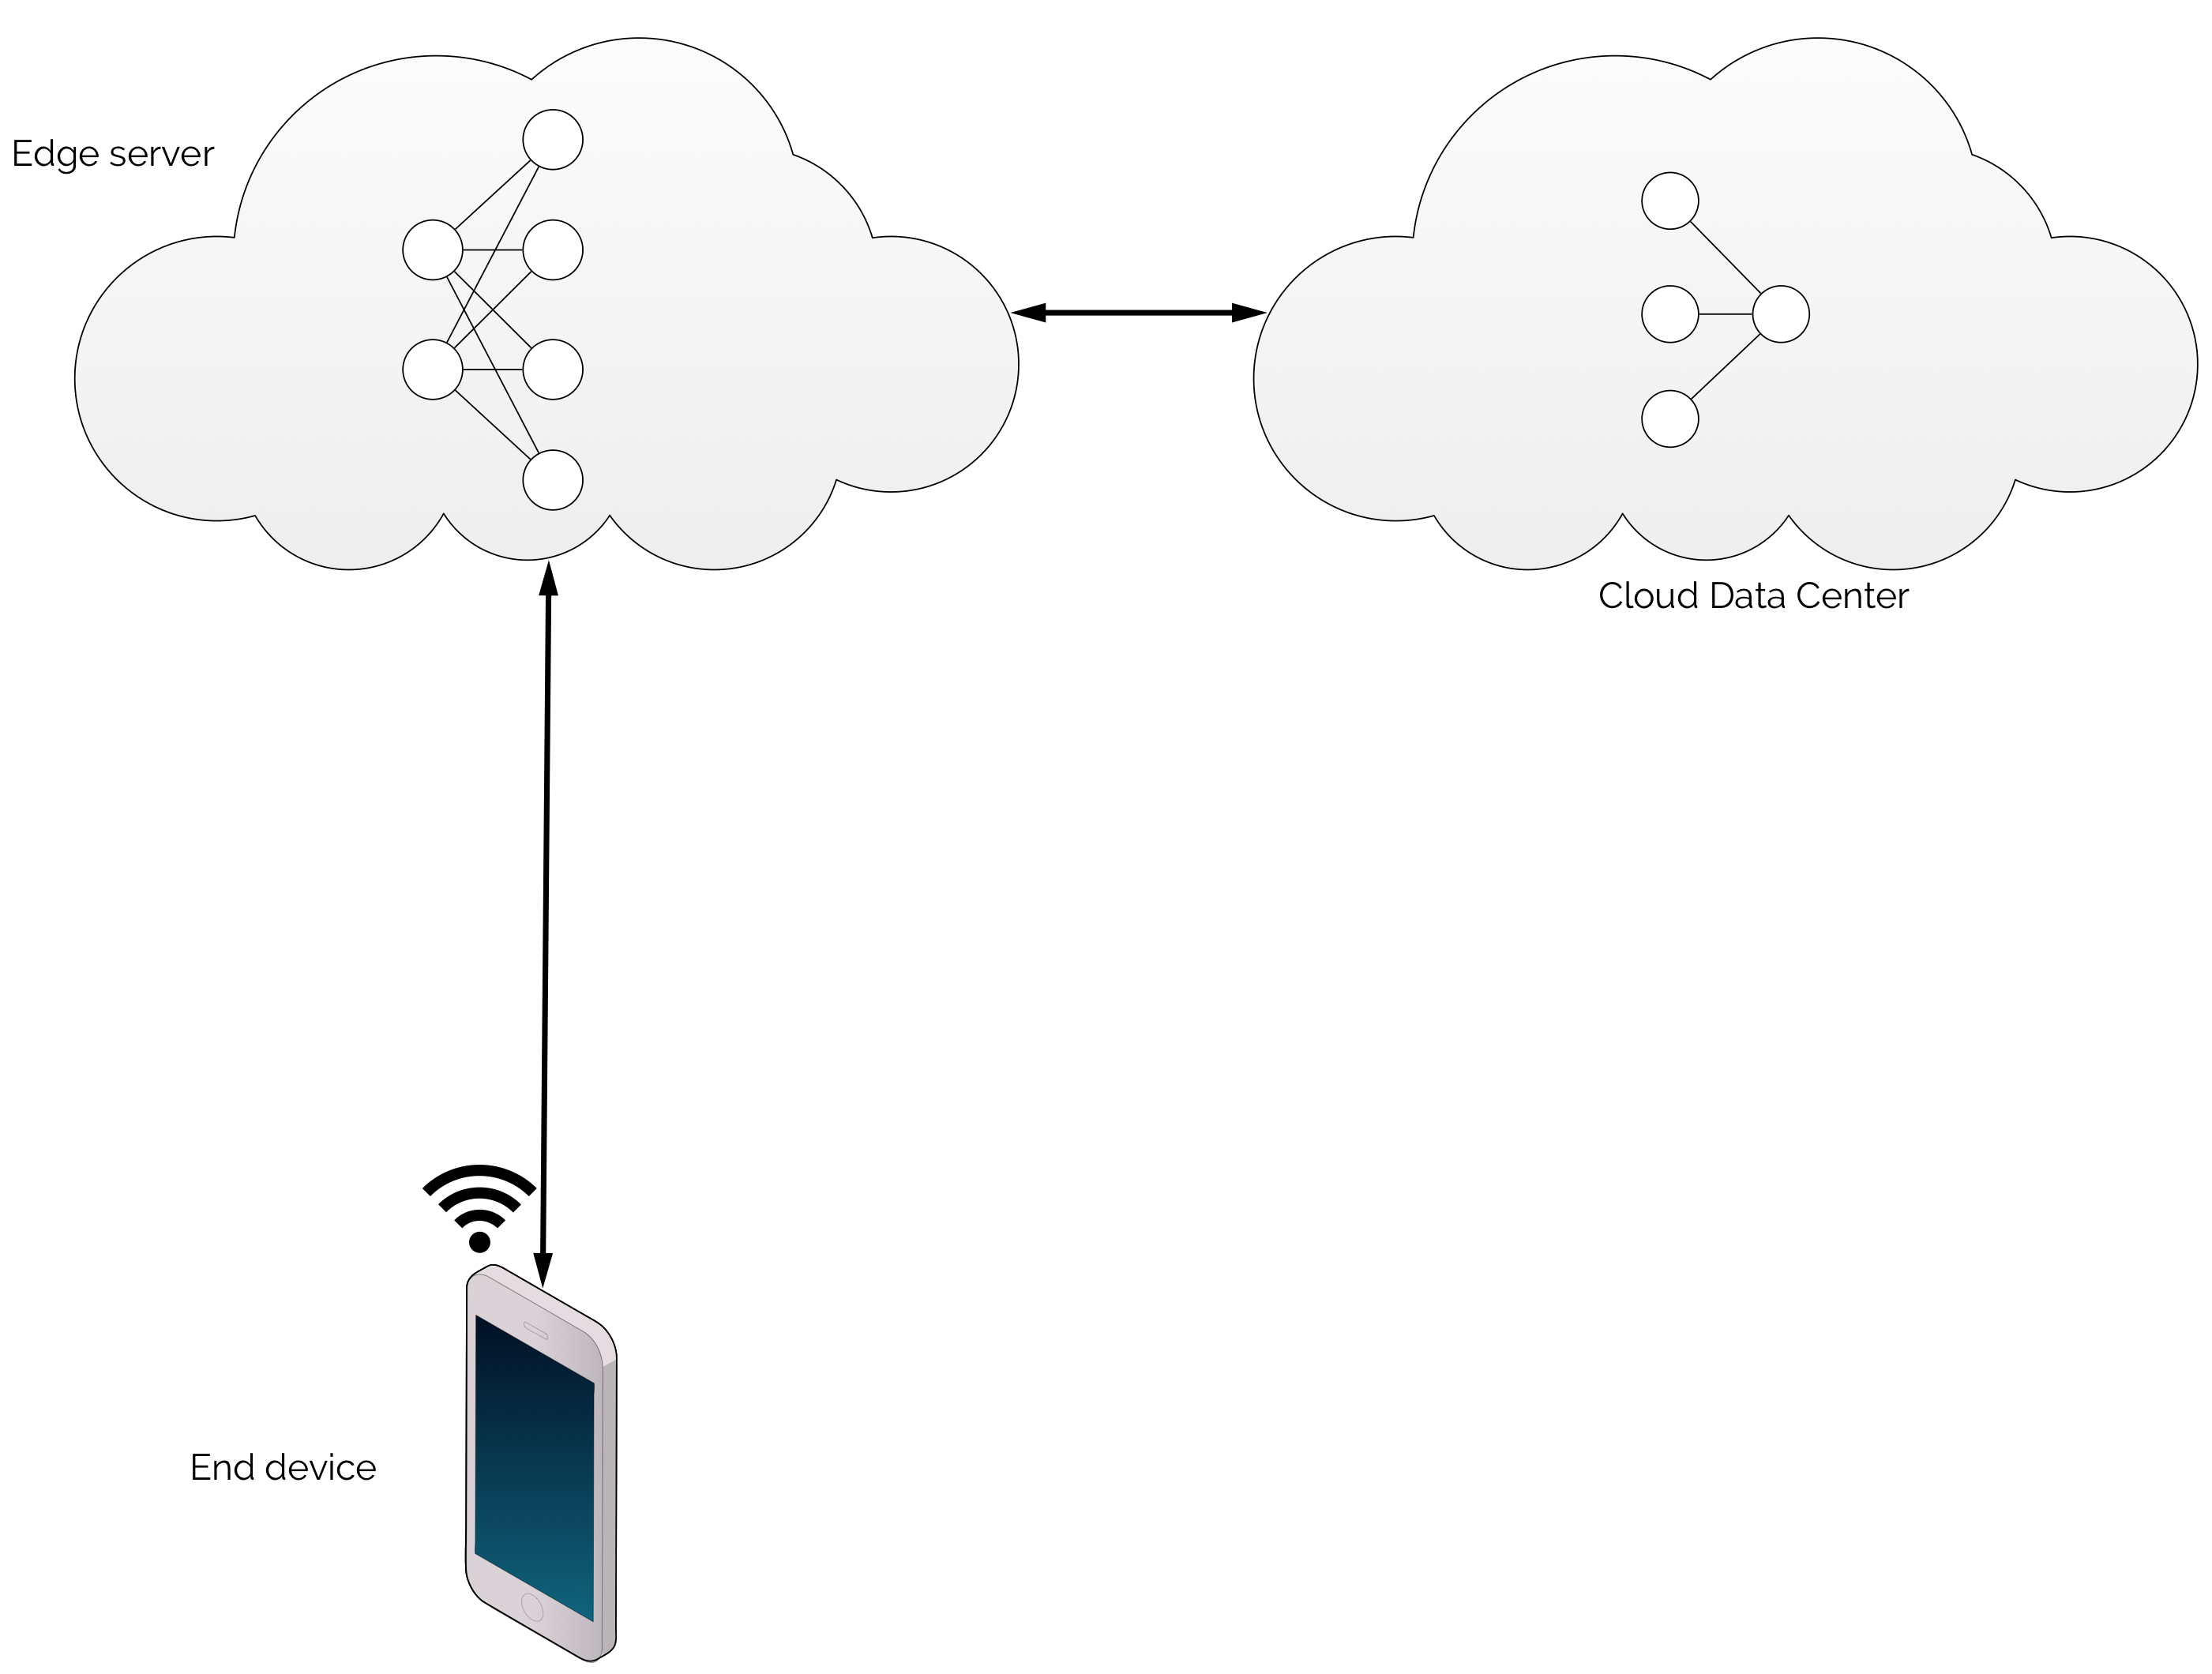
\includegraphics[width=.37\linewidth]{figures/models/edge_cloud}}
	\caption[Edge-centric architectures]{Edge Architectures: \protect\subref{fig:device-based} device only execution, \protect\subref{fig:edge-based} edge only execution,\protect\subref{fig:edge-device-mode} edge and device partially execution, \protect\subref{fig:edge-cloud-mode} edge and cloud partially execution. }
\end{figure}

\begin{description}
	\item[Device-based Mode]
	 end device obtain model from edge server. The end-device then acquires input data and performs model inference. Since all computation is done on the end device, performance is solely reliant on the end device's computing resources. 
	
	\item[Edge-based Mode] end device acquires input data. The input data is transferred to an edge server, which performs model inference and send the prediction results to the end device. The performance relies on edge server computing resources and network bandwidth.
	\item[Edge-Device Mode] end device acquires input data and performs partially model inference. The intermediate data is transferred to an edge server which finalizes model inference. The performance relies on end device's and edge server computing resource, network bandwidth and edge server workload. 
	\item[Edge-Cloud Mode] resemble edge-device mode, however the model inference task is now partitioned between edge server and cloud data centers. The model is now reliant on edge server and data center computing resources, but even more reliant on \gls{wan} transmission rate between edge and cloud. 
\end{description}

\newpage
\subsection{Edge Architectures}
 
\begin{minipage}{0.65\linewidth}
	\textbf{\textsc{Device-based}}
	
	The model is obtained by the end device from the edge server. The end device then acquires input data and performs model inference. Since all computation is done on the end device, performance is solely reliant on the end device's computing resources. 
\end{minipage}%
\hfill
\begin{minipage}{0.3\linewidth}
	\centering
	\begin{figure}
		\centering
		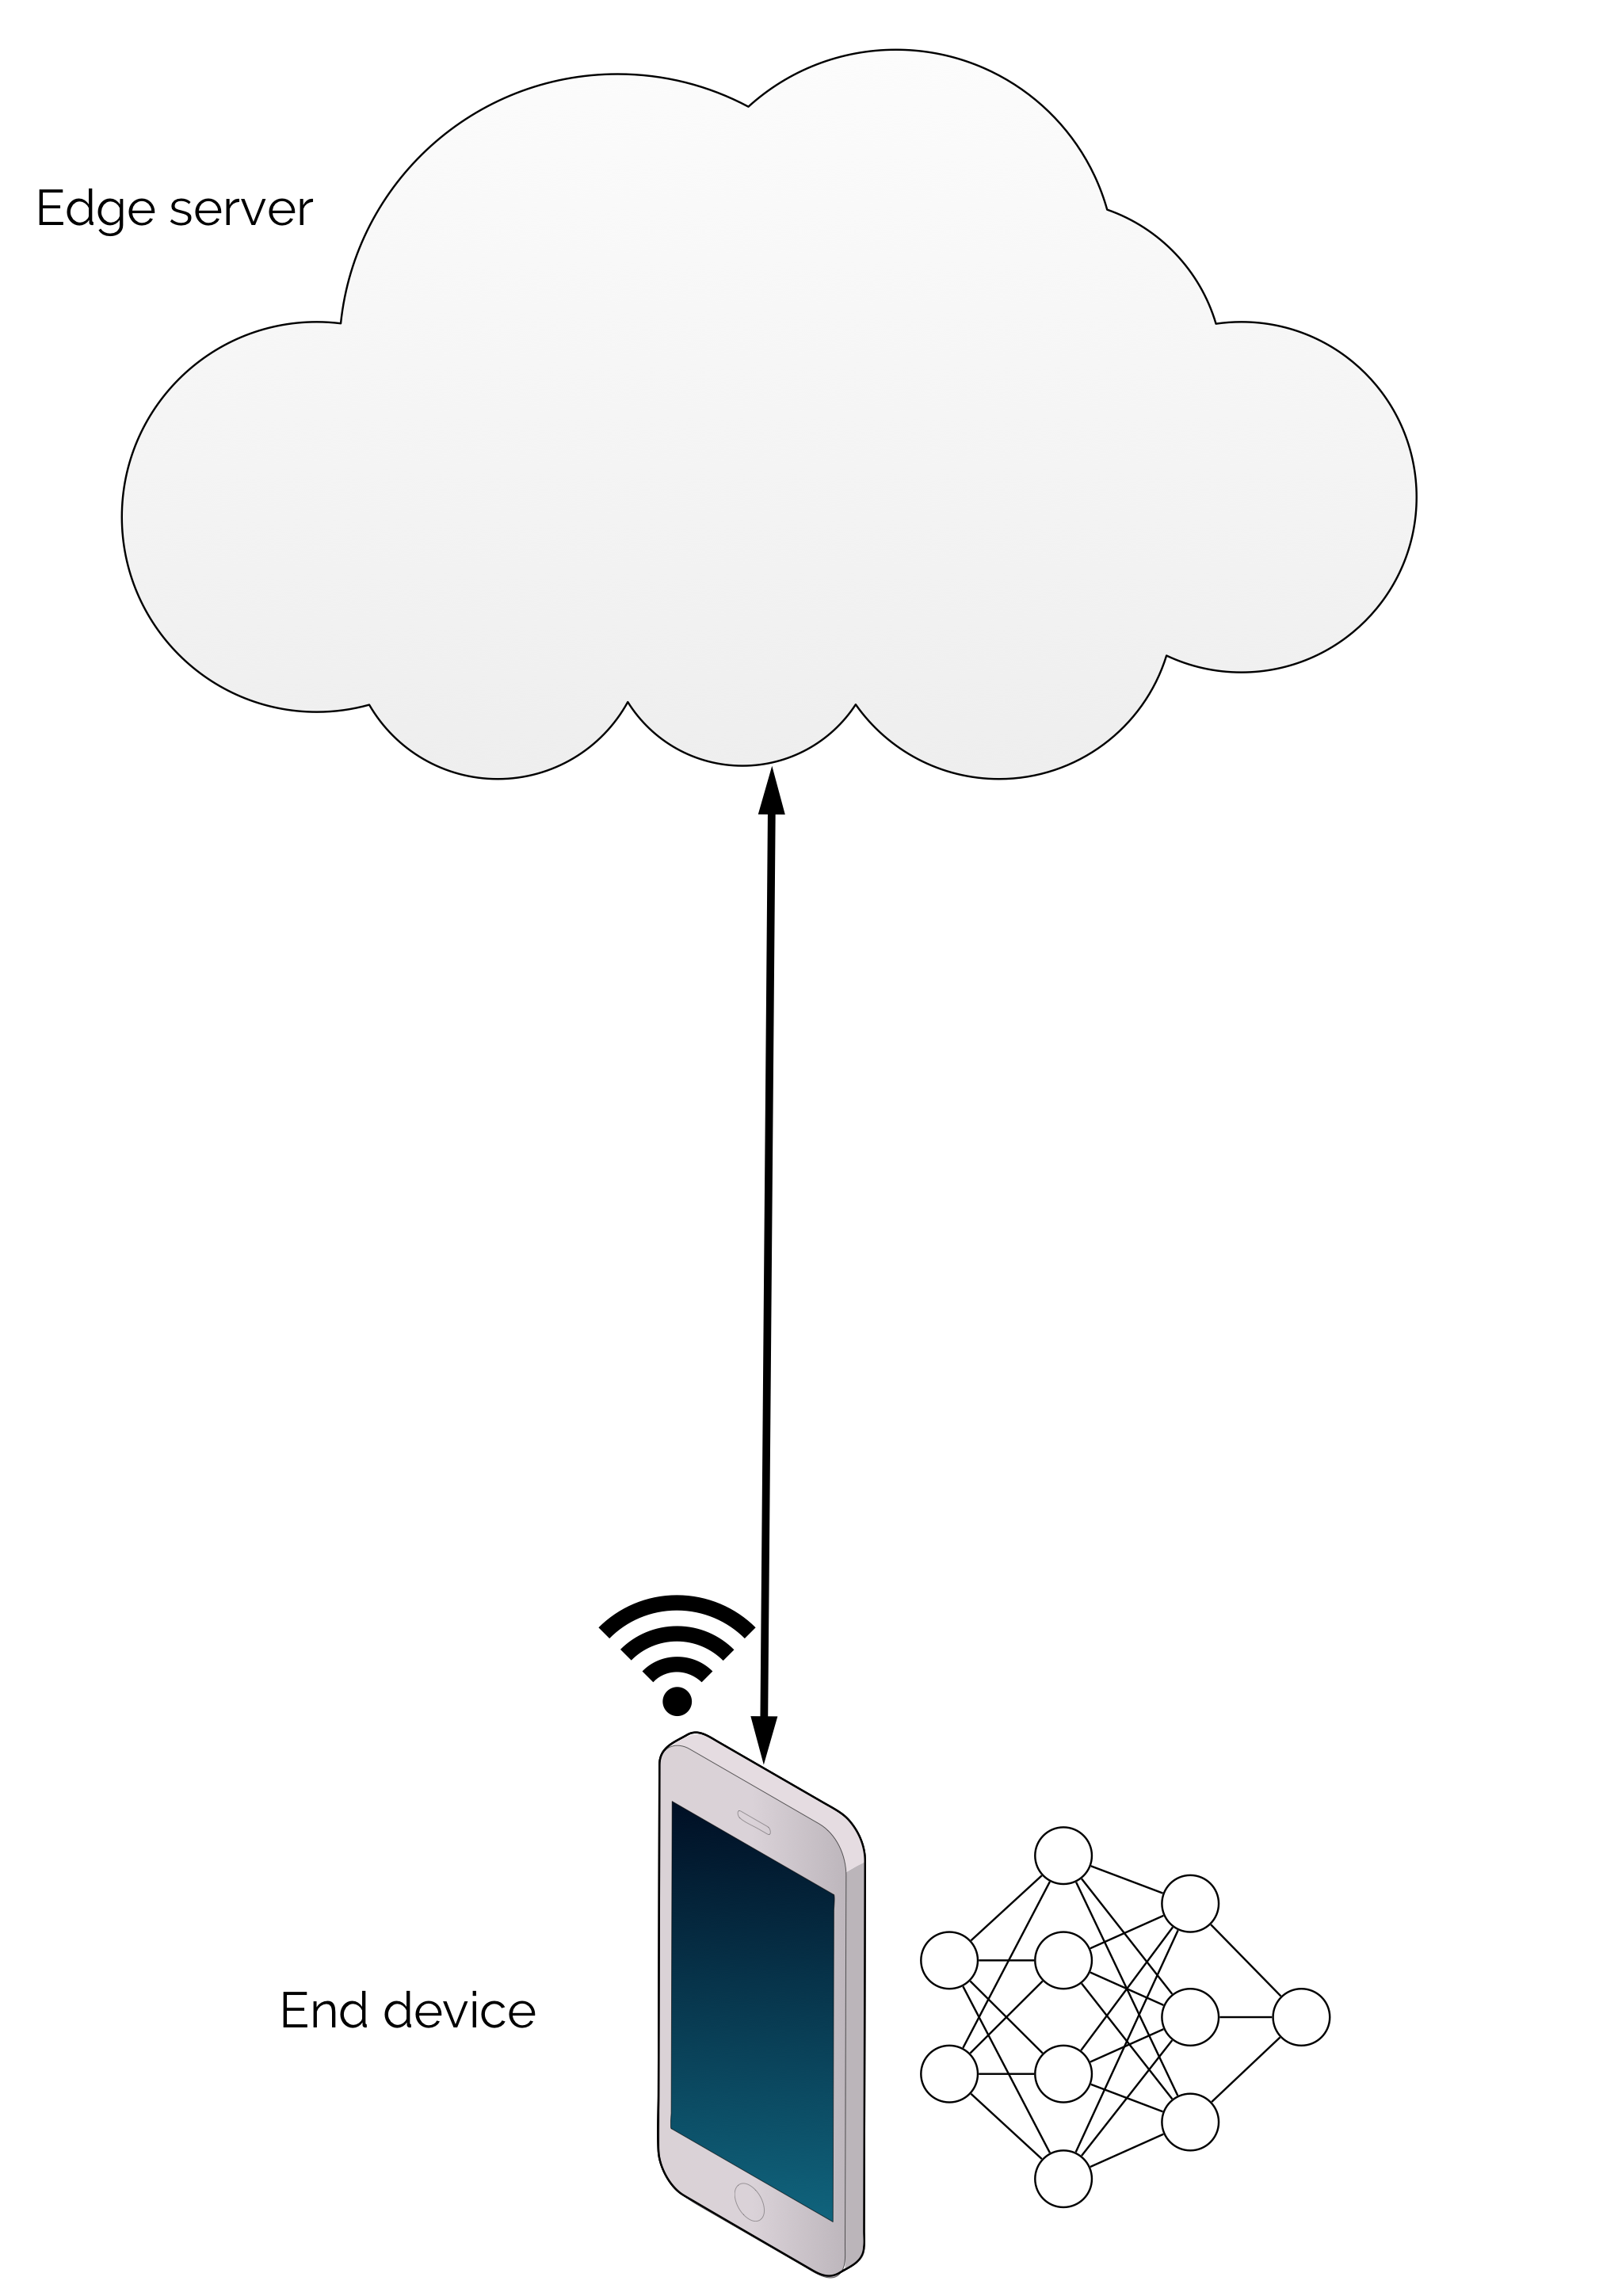
\includegraphics[width=\linewidth]{figures/models/device}
		\caption[Device-based]{Device-based}
	\end{figure}
\end{minipage}

\begin{minipage}{0.3\linewidth}
	\centering
	\begin{figure}
		\centering
		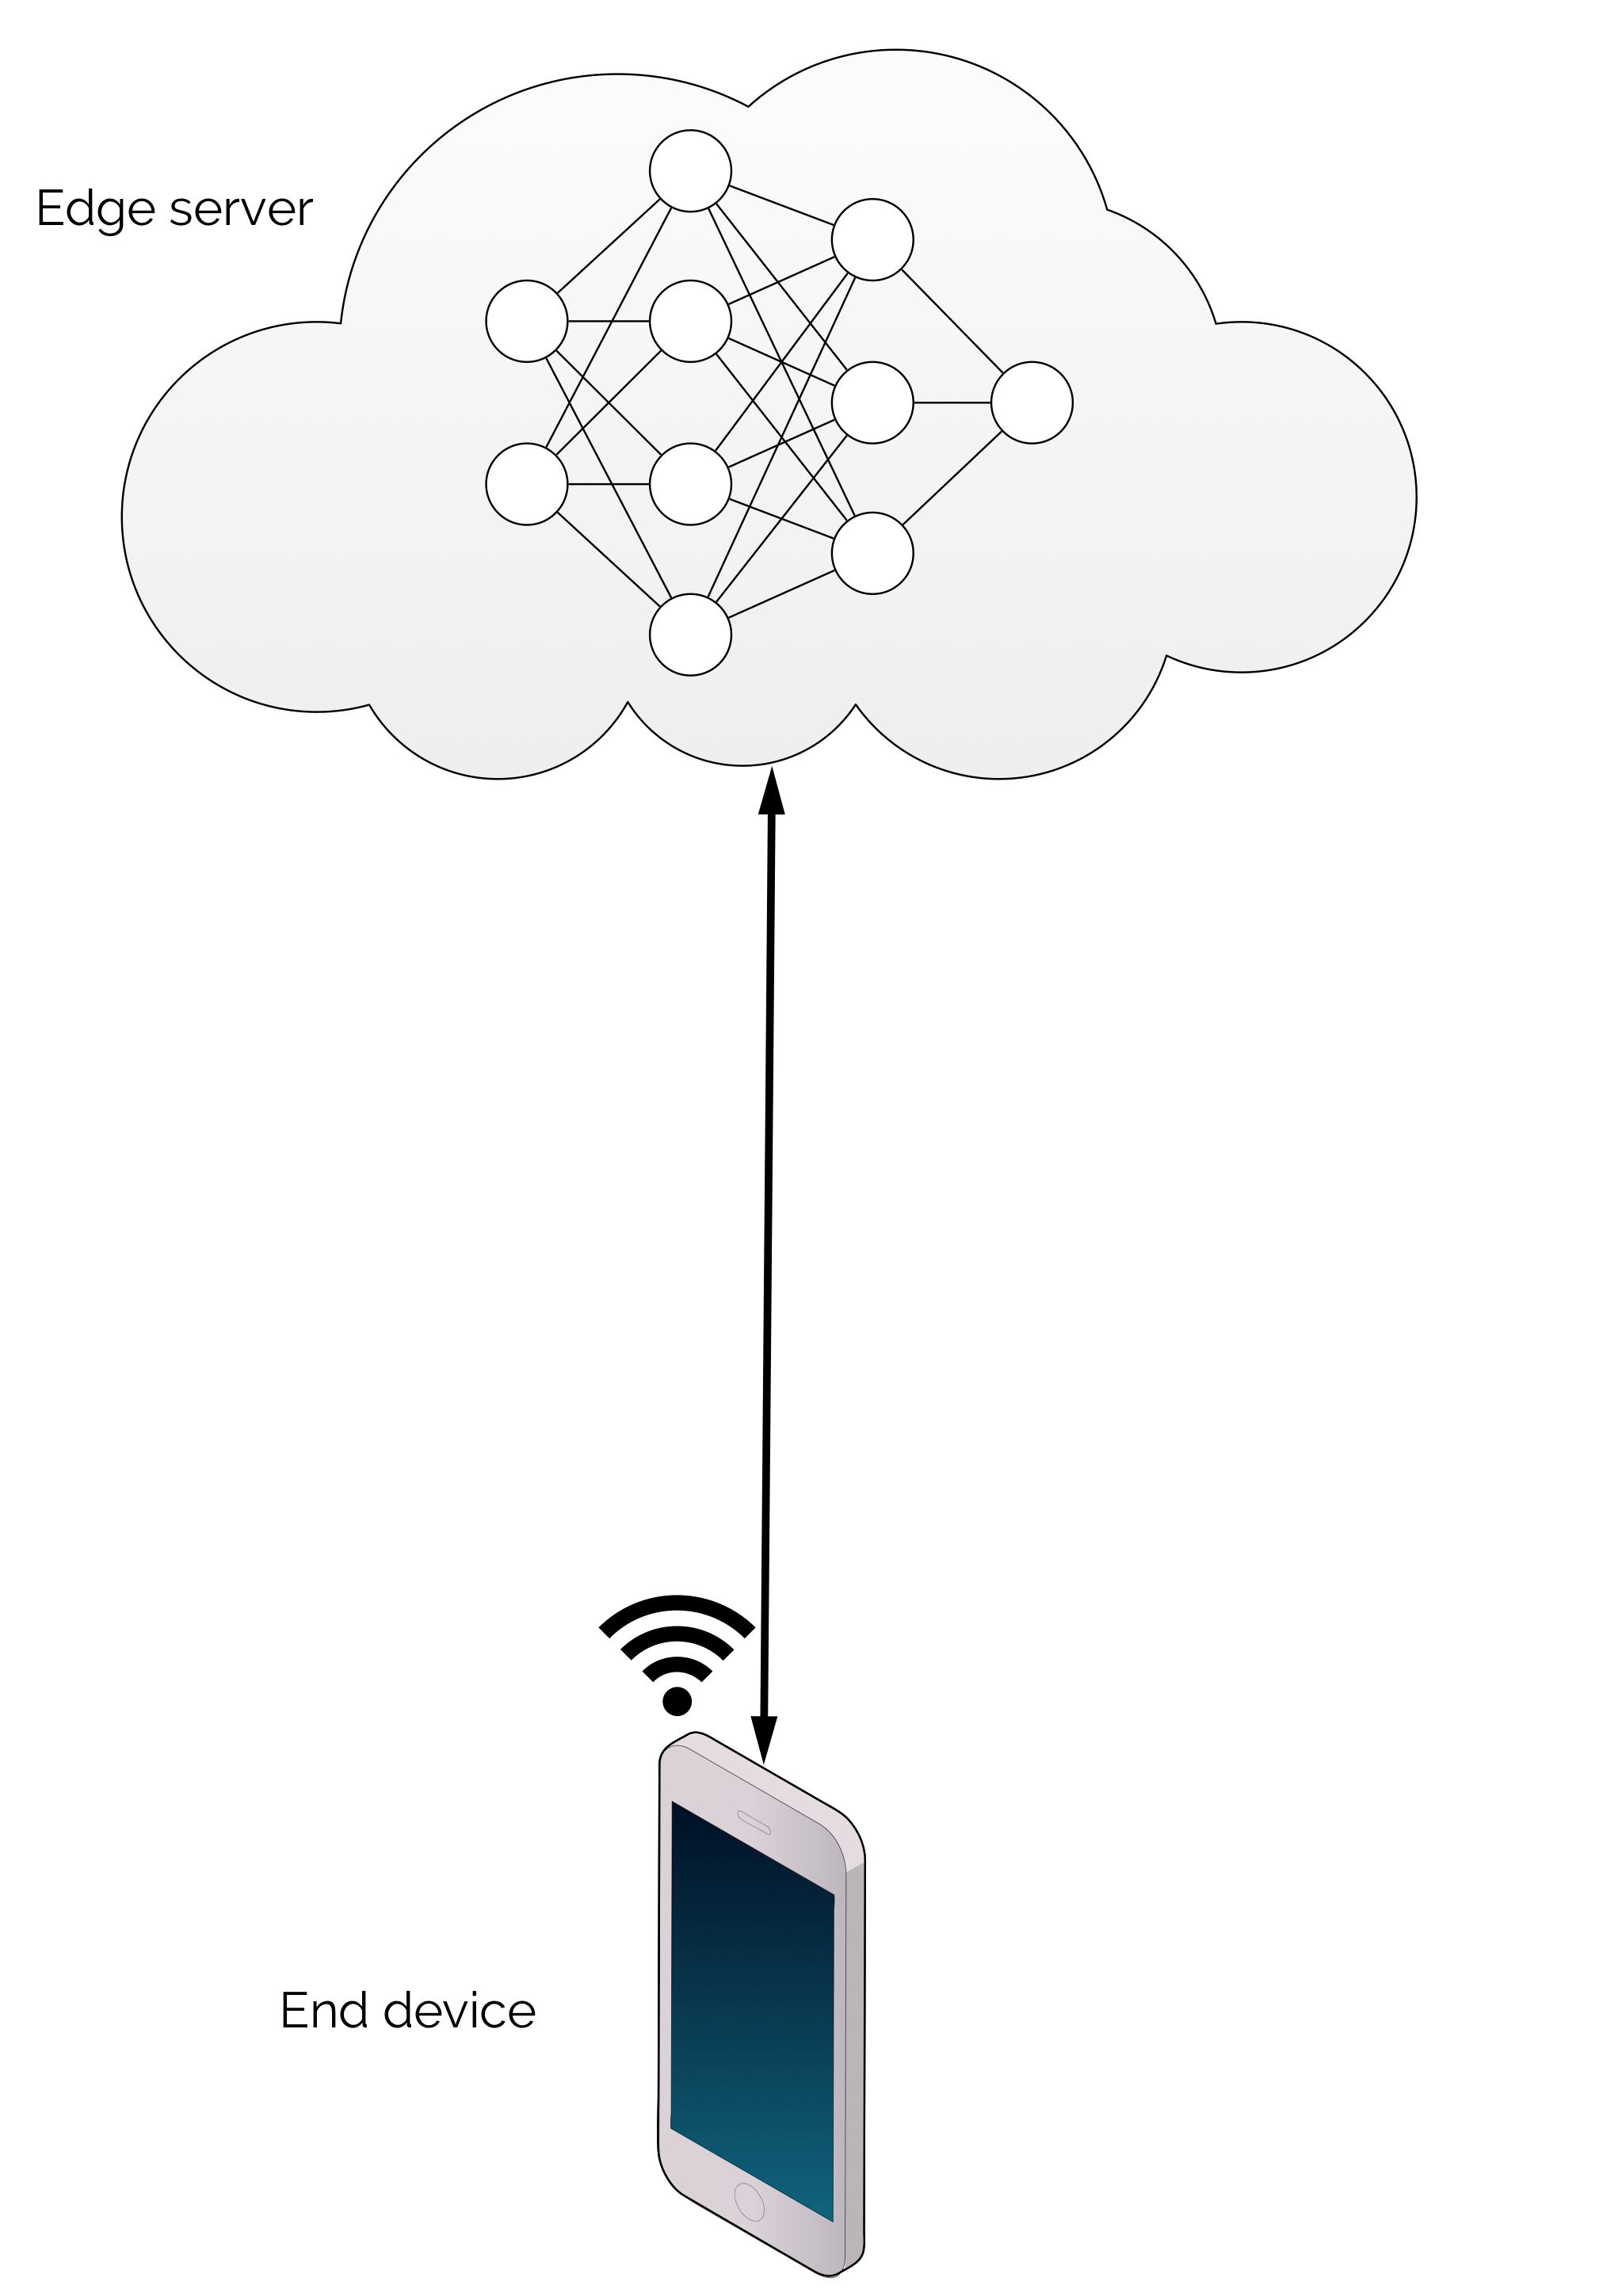
\includegraphics[width=\linewidth]{figures/models/edge}
		\caption[Edge-based]{Edge-based}
	\end{figure}
\end{minipage}
\hfill
\begin{minipage}{0.65\linewidth}
	\textbf{\textsc{Edge-based}}
	
	The end device acquires input data. The input data is transferred to an edge server, which performs model inference and send the prediction results back to the end device. The performance relies on edge server computing resources and the available network bandwidth between end device and edge server. 
\end{minipage}
\begin{minipage}{0.65\linewidth}
	\textbf{\textsc{Collaborative Edge}}
	
	The end device acquires input data and performs partially model inference. The intermediate data is transferred to an edge server which finalizes model inference. The performance relies on the computing resource of both the end device and the edge server and edge server workload, as well as available network bandwidth between end device and edge server. 
\end{minipage}%
\hfill
\begin{minipage}{0.3\linewidth}
	\centering
	\begin{figure}
		\centering
		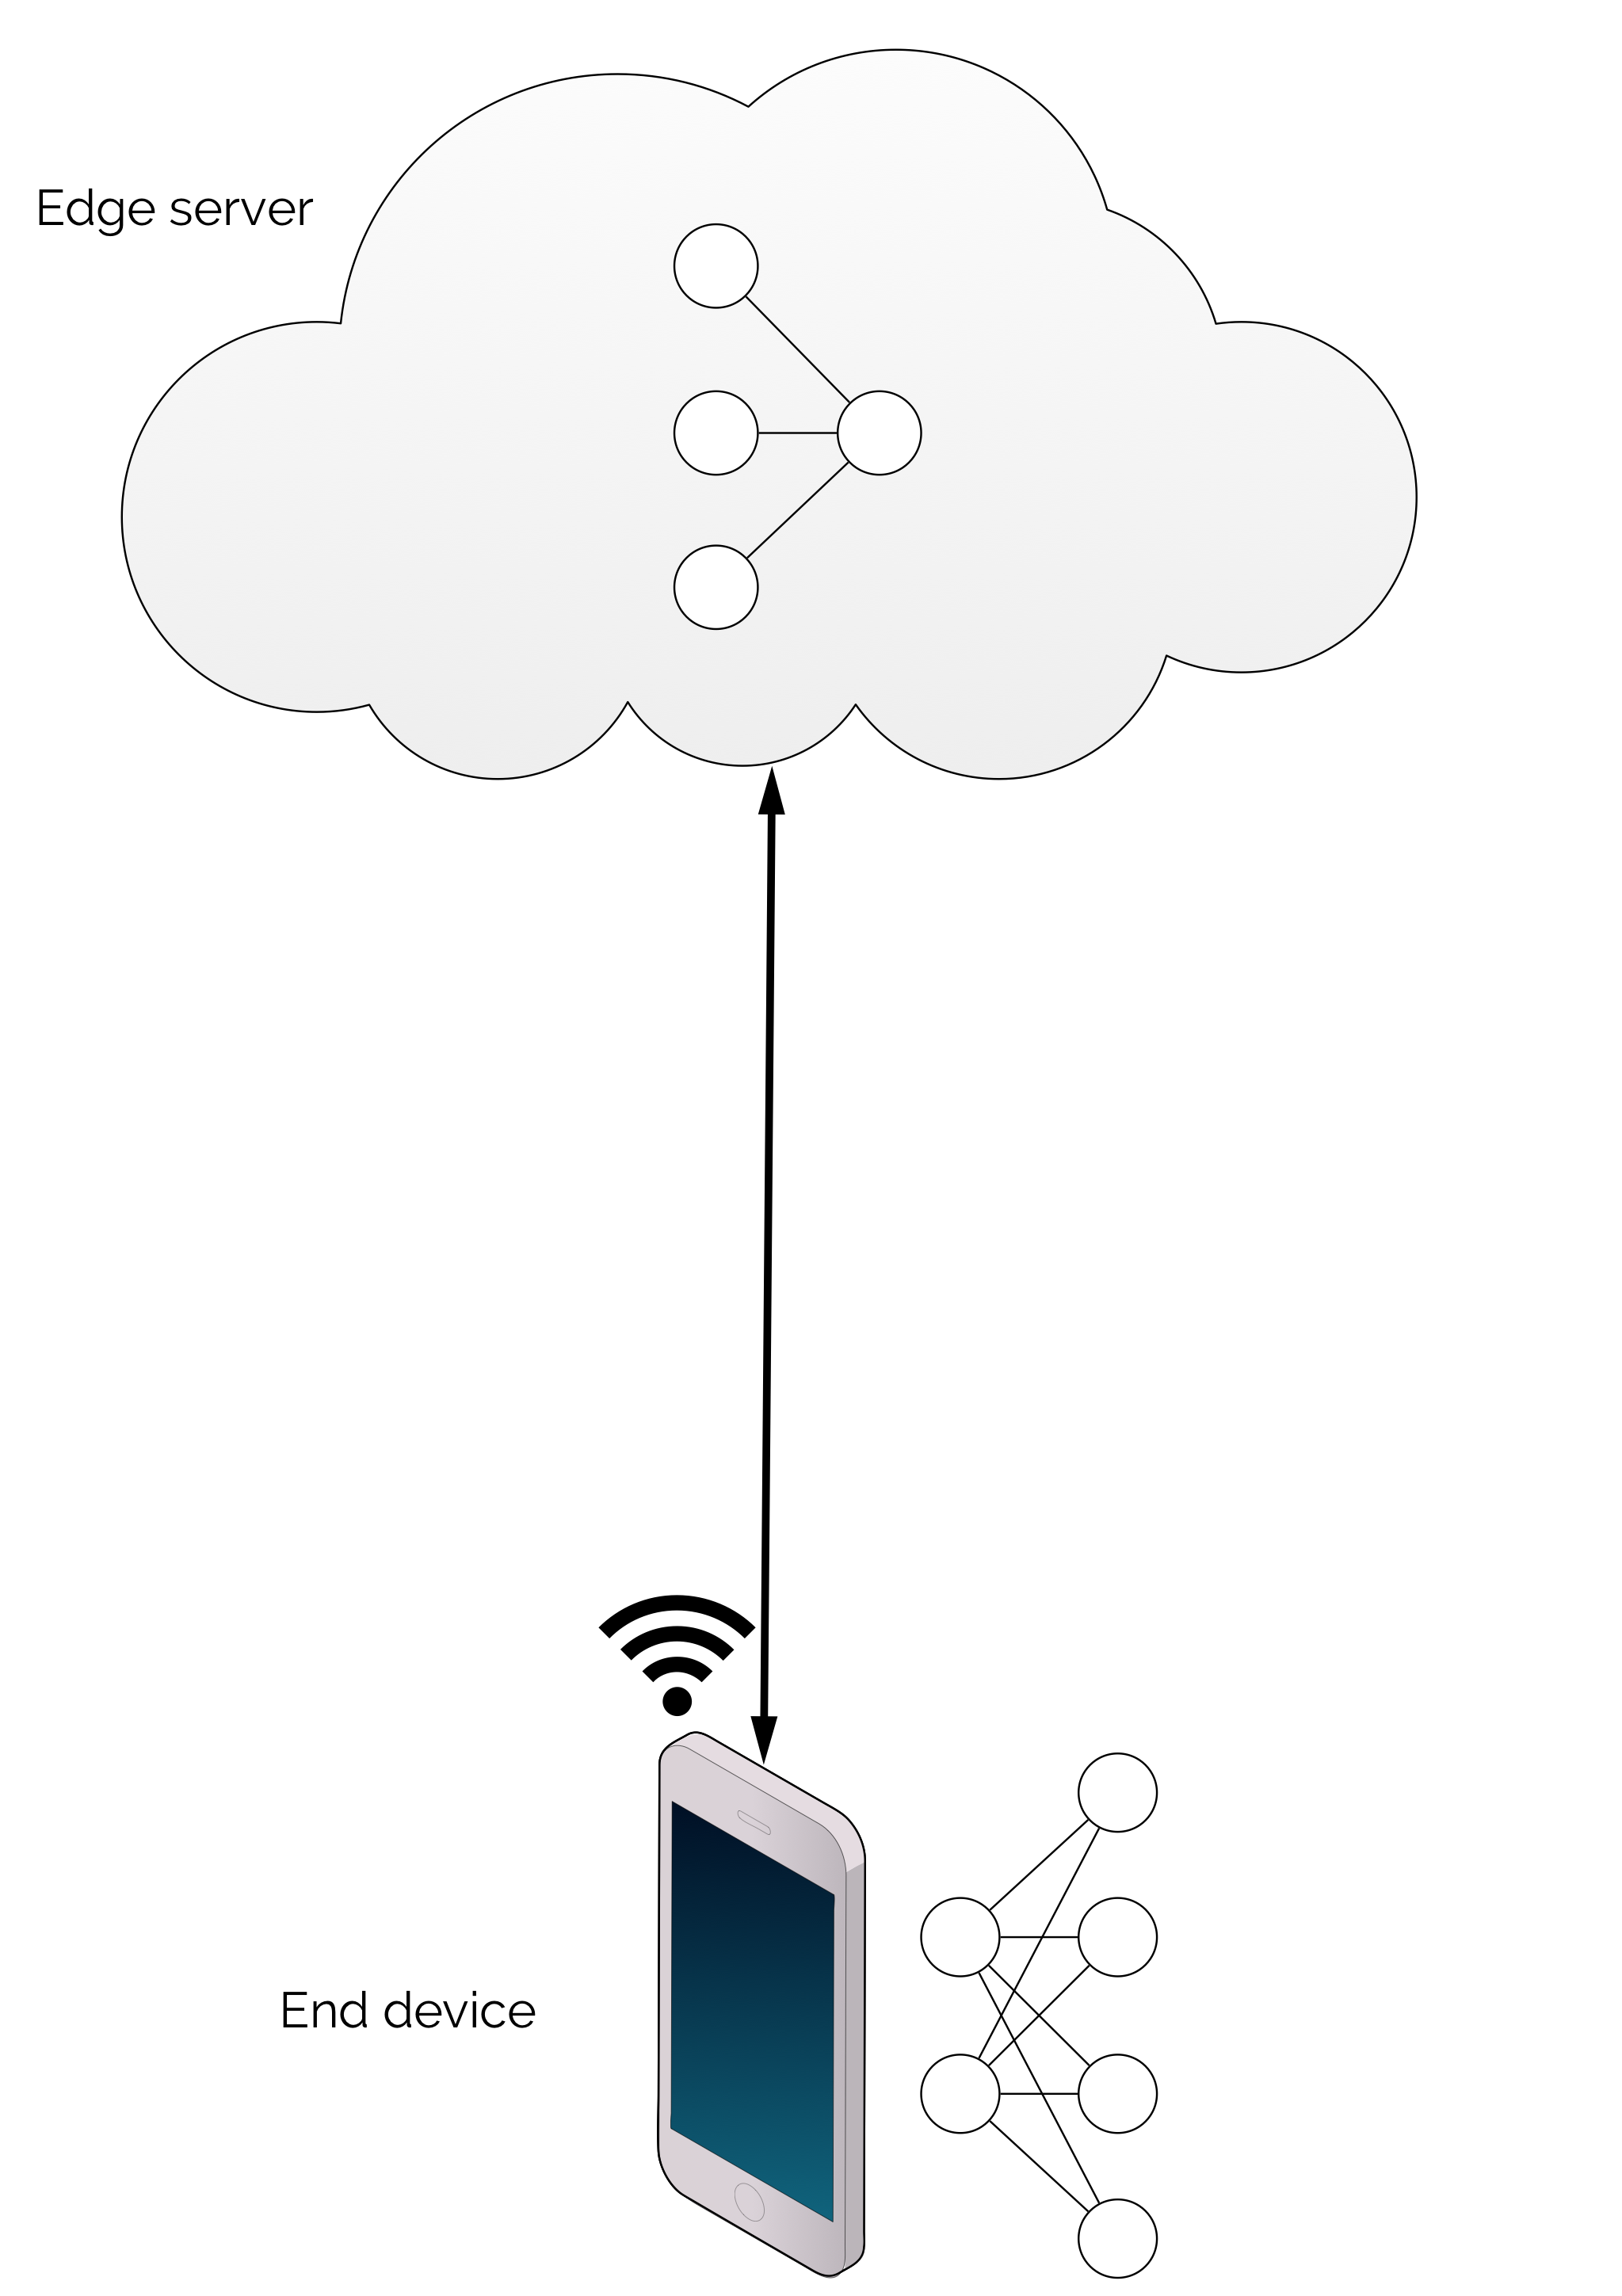
\includegraphics[width=\linewidth]{figures/models/edge_device}
		\caption[Collaborative Edge]{Collaborative Edge}
	\end{figure}
\end{minipage}

\begin{minipage}{0.5\linewidth}
	\centering
	\begin{figure}
		\centering
		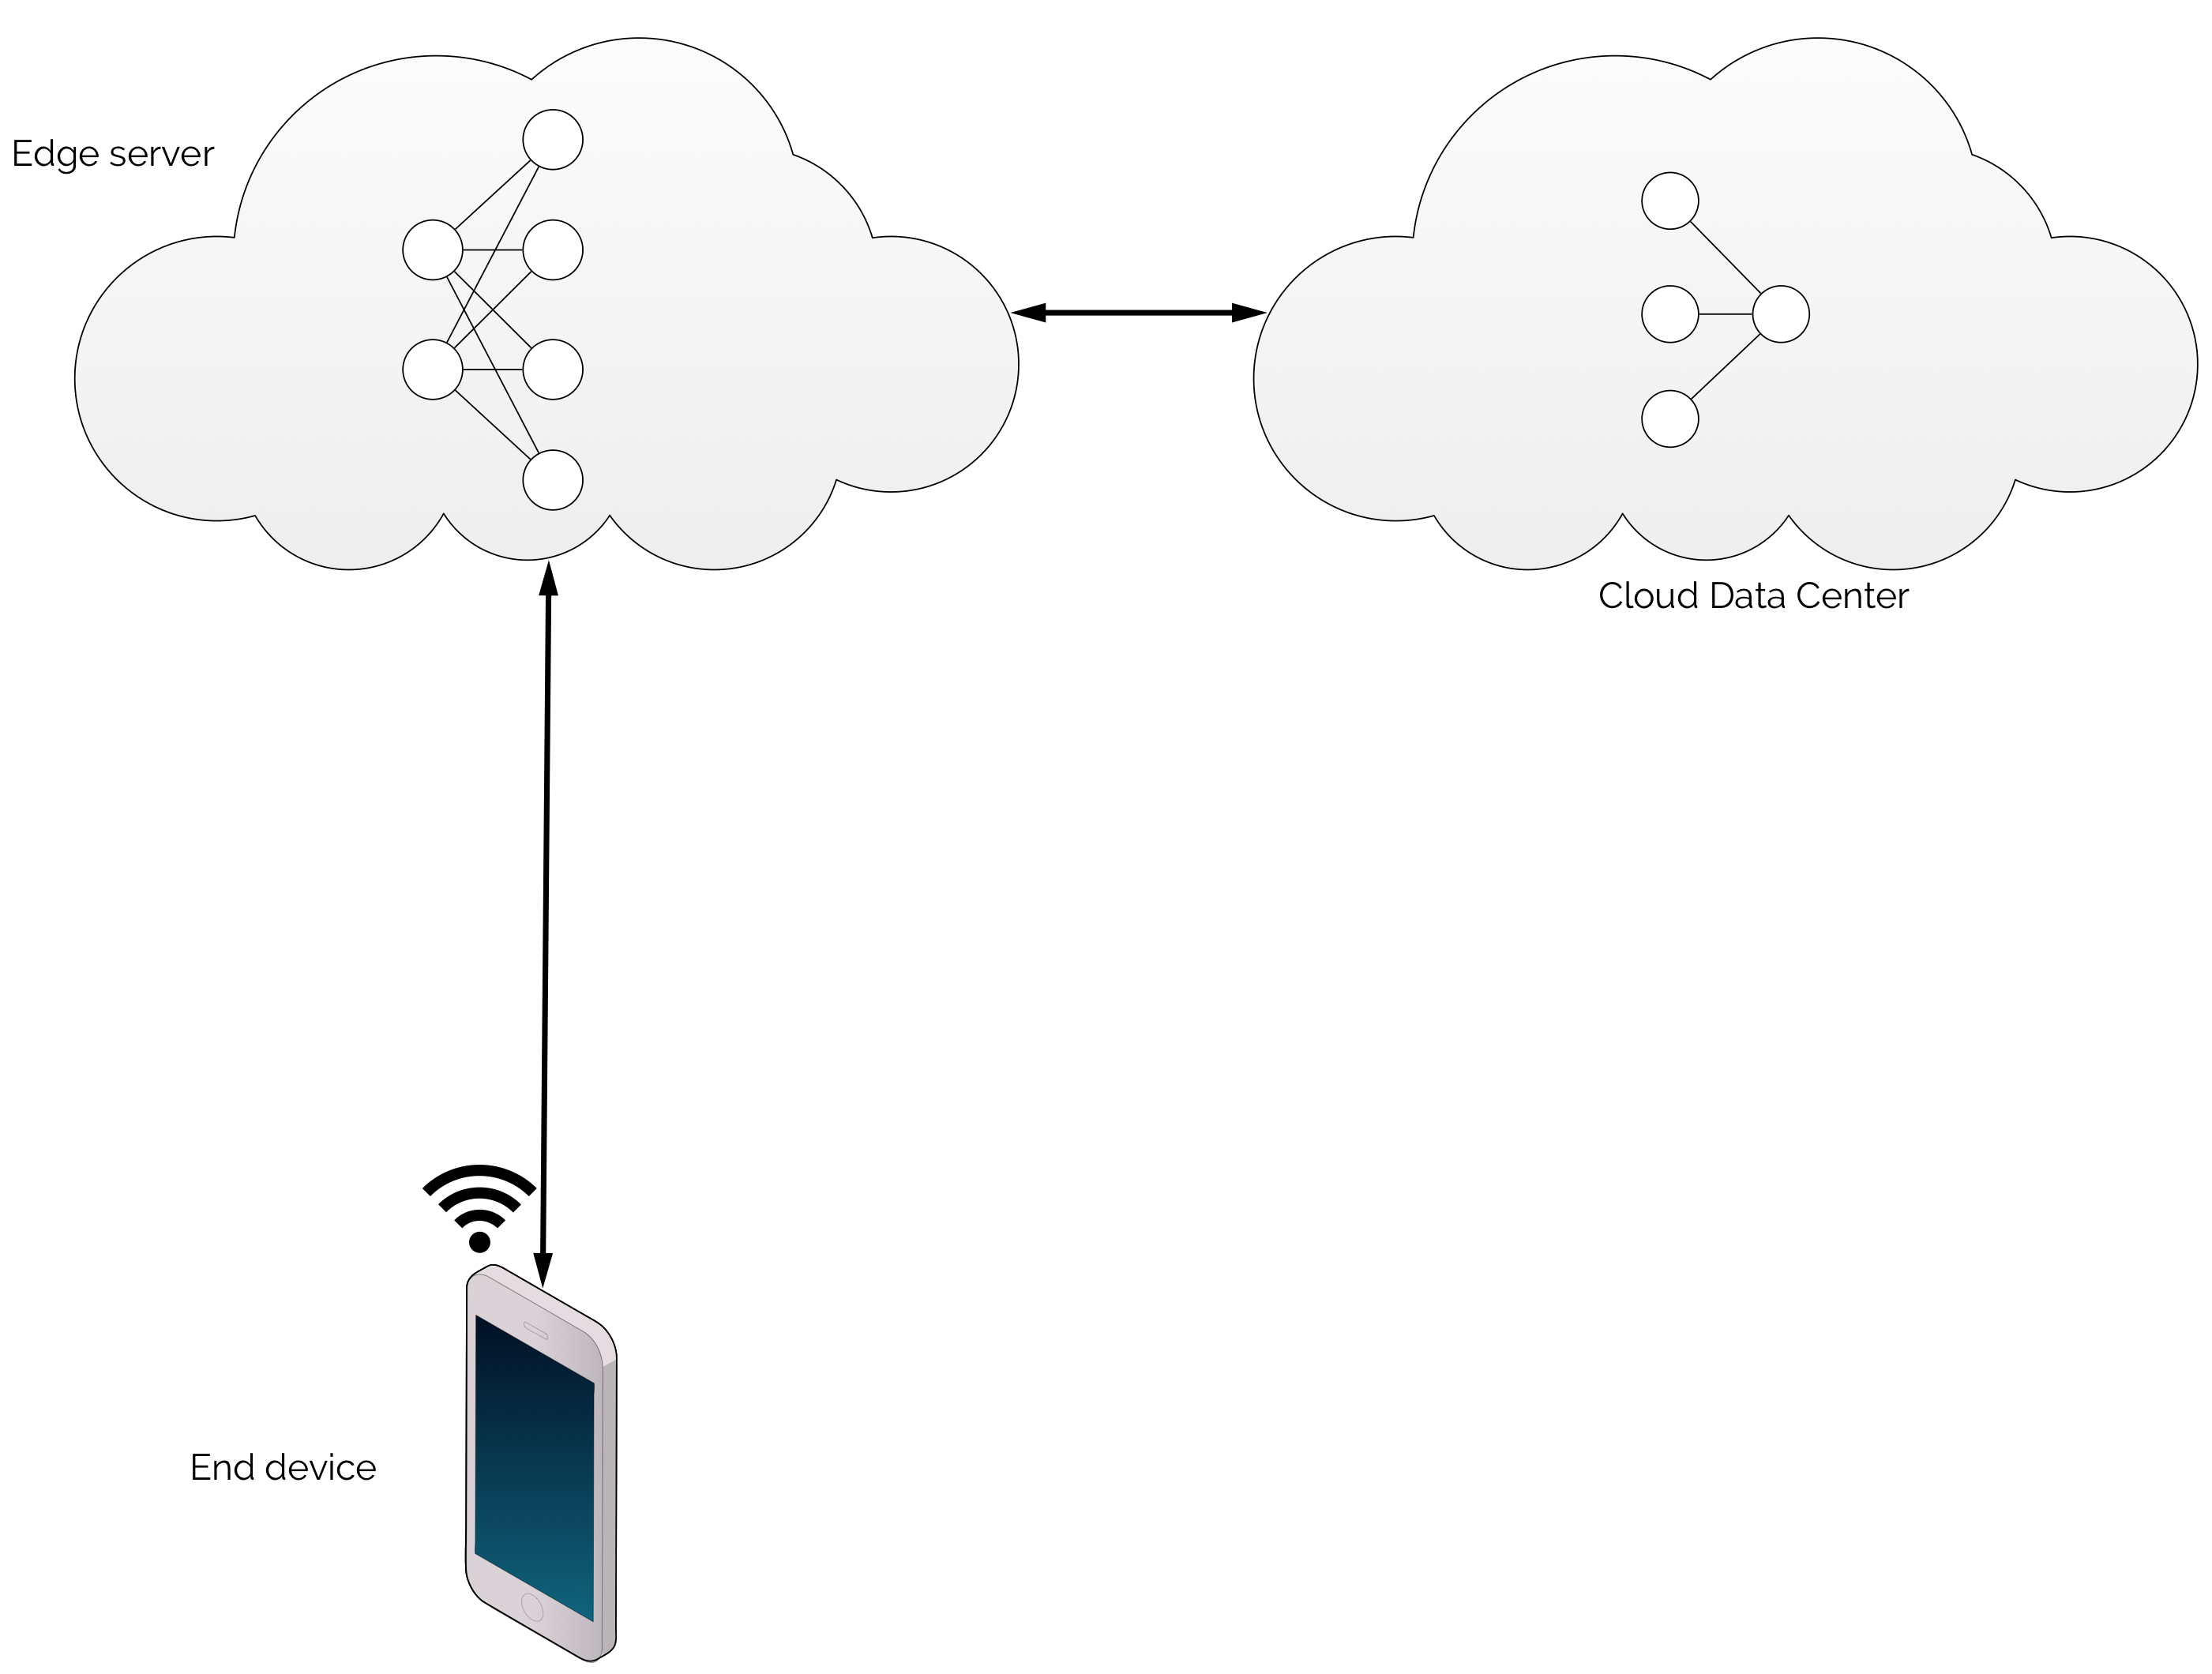
\includegraphics[width=\linewidth]{figures/models/edge_cloud}
		\caption[Collaborative Edge-Cloud]{Collaborative Edge-Cloud}
	\end{figure}
\end{minipage}
\hfill
\begin{minipage}{0.45\linewidth}
	\textbf{\textsc{Collaborative Edge-Cloud}}
	
	resemble edge-device mode, however the model inference task is now partitioned between edge server and cloud data centers. The model is now reliant on edge server and data center computing resources, but even more reliant on \gls{wan} transmission rate between edge and cloud.
\end{minipage}

Over recent years interest research in reducing inference time have grown. In the next section related work will be explained.  


%Recent years breakthrough within \gls{dl} have led to a dramatic increase in the amount of \gls{ai} applications and services, such as personal assistants, recommendation systems and surveillance systems. Combined with the development of mobile computing and \gls{iot}, where billions of device are getting connected to the internet. Traditionally data for \gls{ai} applications and services are generated by the devices and transferred to large data centers for computation.    To fully unleash the power of \gls{ai} applications and services \gls{ei} or edge \gls{ai} have become an interesting research area. \gls{ei} have potential to reduce the 